% ------------------------------
    \section{Results and discussion} % (fold)
    \label{sec:results}
    % ------------------------------
    In \cref{tab:energiesCASSCF}, the MCSCF energies computed with each approximated
    2-RDM given in \cref{sec:approximated-2rdms}, together with the absolute
    errors, are tabulated for the CASSCF calculation corresponding to the input file
    (file \ref{lst:CASSCF-input}) of the \cref{sec:appendix-dalton}.
    The performed calculations for this input correspond to CASSCF(8,8)/cc-pVDZ
    with 1 inactive orbital.
    The energy error is a direct measurement of the performance of each approximation.

    Also, the Minkowski distances of order $p=4$ computed with \cref{eq:minkowski-distance}
    are tabulated in \cref{tab:minkowski}.
    This metric serves as a direct way to compare each approximated 2-RDM with the
    exact one which, along with the MCSCF energy, serves to gut the functioning of
    the 2-RDMs.

    \begin{table}[b!]
        \scriptsize
        \ra{1.2} % Spacing btween lines of table
        \caption{CASSCF energies and absolute errors, in hartrees, for the LS,
        BBC1, BBC2, BBC3 and BBC3M approximations.}
        \label{tab:energiesCASSCF}
        \centering
        \begin{tabular}{@{}ccccccccccc@{}}
            \toprule
     & \multicolumn{2}{c}{LS} & \multicolumn{2}{c}{BBC1} & \multicolumn{2}{c}{BBC2} & \multicolumn{2}{c}{BBC3} & \multicolumn{2}{c}{BBC3M} \\
     \cmidrule(lr){2-3} \cmidrule(lr){4-5} \cmidrule(lr){6-7} \cmidrule(lr){8-9} \cmidrule(lr){10-11}
            $d$, \AA & $E$, Ha & $\Delta E$ & $E$, Ha & $\Delta E$ & $E$, Ha & $\Delta E$ & $E$, Ha & $\Delta E$ & $E$, Ha & $\Delta E$ \\
            \midrule
            0.5 & -60.2947   & 0.13e-09    & -60.2947     & 0.13e-09      & -60.2947     & 0.13e-09      & -64.8410     & 0.45e+01      & -60.2947     & 0.13e-09     \\
            1.0 & -69.9020   & 0.33e-10    & -69.9020     & 0.33e-10      & -69.9020     & 0.33e-10      & -74.5575     & 0.47e+01      & -69.9020     & 0.33e-10     \\
            1.5 & -71.9914   & 0.13e-11    & -71.9914     & 0.13e-11      & -71.9914     & 0.13e-11      & -76.6761     & 0.47e+01      & -71.9914     & 0.13e-11     \\
            2.0 & -72.8738   & 0.15e-10    & -72.8738     & 0.15e-10      & -72.8738     & 0.15e-10      & -77.5792     & 0.47e+01      & -72.8738     & 0.15e-10     \\
            2.5 & -73.2204   & 0.35e-11    & -73.2204     & 0.35e-11      & -73.2204     & 0.35e-11      & -77.9279     & 0.47e+01      & -73.2204     & 0.35e-11     \\
            3.0 & -73.3153   & 0.46e-10    & -73.3153     & 0.46e-10      & -73.3153     & 0.46e-10      & -78.0228     & 0.47e+01      & -73.3153     & 0.46e-10     \\
            3.5 & -73.2969   & 0.50e-10    & -73.2969     & 0.50e-10      & -73.2969     & 0.50e-10      & -78.0176     & 0.47e+01      & -73.2969     & 0.50e-10     \\
            4.0 & -73.2486   & 0.37e-10    & -73.2486     & 0.37e-10      & -73.2486     & 0.37e-10      & -77.9760     & 0.47e+01      & -73.2486     & 0.37e-10     \\
            \bottomrule
        \end{tabular}
    \end{table}

    \begin{table}[b!]
        \ra{1.2} % Spacing btween lines of table
        \caption{Minkowski distances of order $p = 4$ for the LS, BBC1, BBC2, BBC3
        and BBC3M approximations.}
        \label{tab:minkowski}
        \centering
        \begin{tabular}{@{}ccccccc@{}}
            \toprule
            $d$, \AA    & LS       & BBC1     & BBC2     & BBC3     & BBC3M    \\
            \midrule
            0.5   & 5.9788   & 3.4199   & 3.9839   & 4.0034   & 6.4741   \\
            1.0   & 5.9738   & 3.4174   & 3.9804   & 3.9999   & 6.4664   \\
            1.5   & 5.8923   & 3.3777   & 3.9228   & 3.9424   & 6.3552   \\
            2.0   & 5.9424   & 3.4021   & 3.9584   & 3.9779   & 6.4207   \\
            2.5   & 5.9397   & 3.4008   & 3.9564   & 3.9759   & 6.4170   \\
            3.0   & 5.9135   & 3.3880   & 3.9379   & 3.9574   & 6.3819   \\
            3.5   & 5.8485   & 3.3566   & 3.8917   & 3.9114   & 6.3039   \\
            4.0   & 5.6882   & 3.2811   & 3.7779   & 3.7978   & 6.1611   \\
            \bottomrule
        \end{tabular}
    \end{table}

    Upon examining \cref{tab:energiesCASSCF}, the first thing the reader may notice
    is the low errors obtained for the different approximations.
    This implies two things: first, that the approximations, at least in this case,
    work very well; second, considering that all the approximate 2-RDMs are
    constructed based on the ONs, i.e. the 1-RDMs, it suggests that the 1-RDMs
    used in these calculations are of high quality, which makes sense considering
    the setup and performance of the CASSCF calculation performed in this case.

    This can also be seen in \cref{fig:plot_pdf}, where the MCSCF energies, absolute
    errors and Minkowski distances of order $p=4$ are shown.
    In the first subfigure, it can be seen that all the energies are real close to
    the exact energy except for one: the BBC3 approximation.
    It can also be seen in the second subfigure, where the errors corresponding
    to BBC3 go up to $\sim 10^{10}$ times the errors corresponding to the rest
    of approximations.

    \begin{figure}[tb!]
        \centering
        % 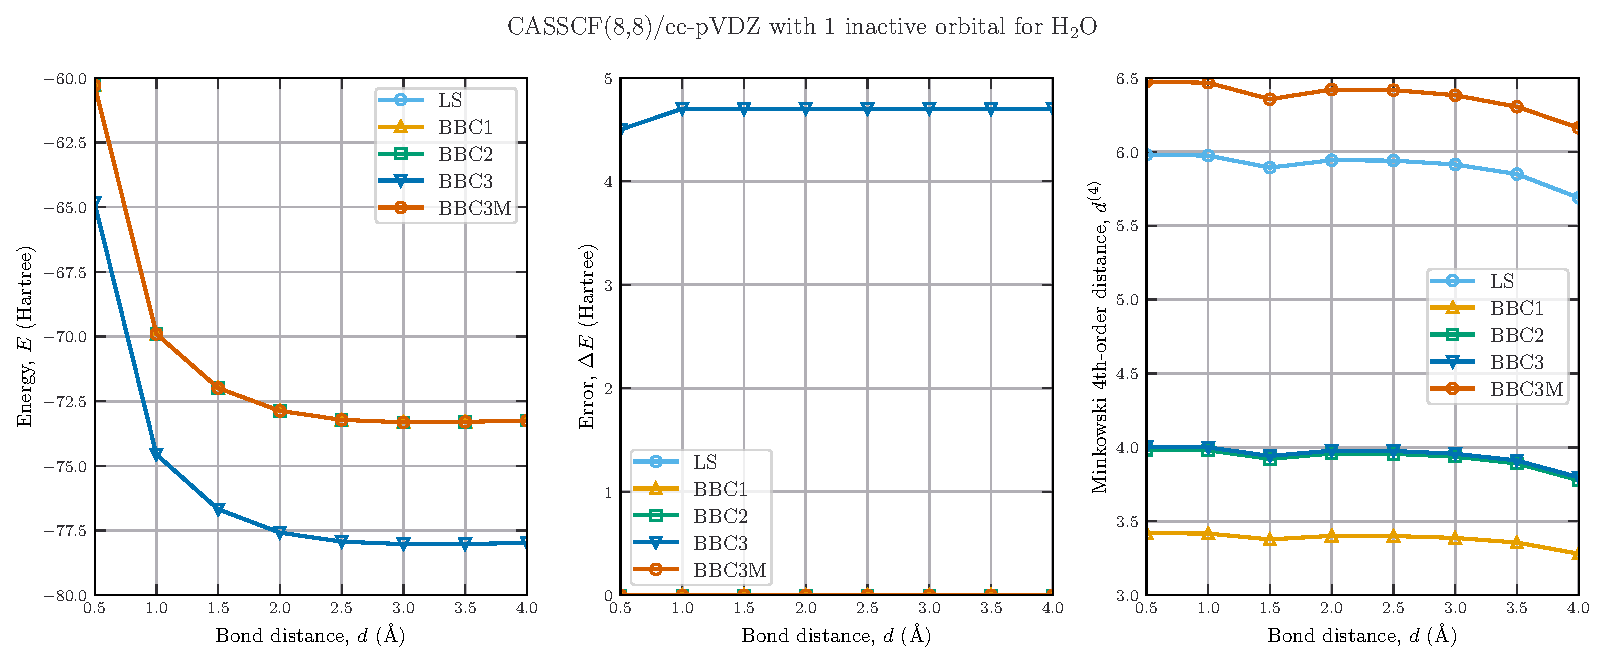
\includegraphics[width=1.0\textwidth]{MCSCF-ccpVDZ.pdf}
        \subimport{figures/}{MCSCF-ccpVDZ.pgf}
        \caption{CASSCF energies, absolute errors and Minkowski distances of order 
        $p=4$ for the LS, BBC1, BBC2, BBC3 and BBC3M approximations.}
        \label{fig:plot_pdf}
    \end{figure}

    This is the result of the main problem discussed in \cref{sec:approximated-Eee},
    the assignment of frontier orbitals.
    In this case, no automatized function was used.
    An orbital $p$ was selected as antibonding if $0 \le n_p \le 0.1$, and as
    bonding if $0.9 \le n_p \le 1$.
    Looking at the results, it can be concluded that this criteria does not perform
    well, but was improved with the modification applied in BBC3M.
    This improvement is noticeable in the third subfigure, where the Minkowski distance
    for BBC3 and BBC3M is noticeable different and, furthermore, the difference
    between BBC2 and BBC3 is not noticeable, meaning that the corrections
    applied to BBC2 leading to BBC3 are not well implemented.
    Also, the BBC3 2-RDM was the only approximated 2-RDM to not fulfill the normalization
    condition, which is a clear indication that important contributions were lost
    with this classification criteria.

    One possible improvement for the classification of bonding and antibonding
    orbitals would be to use the CI coefficients, such that the high-occupation
    orbitals of a relevant configuration (large CI coefficient), associated with
    a decrease of the energy, would be classified as bonding.
    Similarly, a low-occupation orbital of a relevant configuration, associated
    with an increase in the energy, would be classified as antibonding.

    With \cref{tab:minkowski}, and looking at the third subplot of \cref{fig:plot_pdf},
    different values of the Minkowski distance can be observed, eventhough the
    energy errors are very close between all approximations.
    In fact, the Minkowski distance corresponding to BBC3 is lower than that
    corresponding to BBC3M and LS, although the BBC3 approximation is the worst-performing
    approximation.
    This is the main reason why the Minkowski distance is not a performance metric.
    Also, the Minkowski distance for BBC3M is $\sim 4$ times larger than that of
    BBC1, which means that both perform well in this case while being constructed
    differently.

    % Analogous FCI and HF+MP2 calculations have been performed, obtaining very similar
    % results.
    Different order Minkowski distances were computed (see \cref{fig:minkowski-plot}
    in the \cref{sec:appendix-minkowski}), with equivalent results.
    The order $p=4$ is included because, in this case, all distances were
    $0 \le d \le 10$ which is convenient in order to not work with big number.
